\documentclass{article}

\usepackage{graphicx}
\usepackage{url}
\usepackage{natbib}
\usepackage{fancyvrb}
\usepackage{float}

% Definitions
\newcommand\wtfgenes{WTFgenes}
\newcommand\longtitle{WTFgenes: What's The Function of these genes? Static sites for model-based gene set analysis}
\newcommand\shorttitle{WTFgenes}

\newcommand\shortauthors{Christopher J. Mungall and Ian H. Holmes}
\newcommand\longauthors{Christopher J. Mungall$^{\text{\sfb 1}}$ and Ian H. Holmes$^{\text{\sfb 2,3}}$}
\newcommand\authorsaddress{
  $^{\text{\sf 1}}$Environmental Genomics and Systems Biology Division, Lawrence Berkeley National Laboratory, 1 Cyclotron Rd, Berkeley, CA 94720, USA. \\
  $^{\text{\sf 2}}$Department of Bioengineering, University of California, Berkeley, CA 94720, USA. \\
  $^{\text{\sf 3}}$Molecular Biophysics and Integrated Bioimaging Division, Lawrence Berkeley National Laboratory, 1 Cyclotron Rd, Berkeley, CA 94720, USA.
}


\begin{document}

\newcommand\structabs[5]{\maketitle \abstract{#1 #2 #3 Contact: #4}}

\title{\longtitle}
\author{\shortauthors}
\maketitle

\section*{Supplementary Information}

We first reprise the model definition as outlined in the main paper, then outline our extensions and benchmarks.

\subsection*{Review of model}

\begin{figure}
\includegraphics[width=\columnwidth]{model}
\caption{
  \label{fig:model}
  Model-based explanation of observed genes ($O_i$) using ontology terms ($T_j$), following \cite{pmid20172960}.
  Other variables and hyperparameters are defined in the text.
  Circular nodes indicate continuous-valued variables or hyperparameters;
  square nodes indicate discrete-valued (boolean) variables.
  Dashed lines indicate deterministic relationships;
  shaded nodes indicate observations.
  Plates (rounded rectangles) indicate replicated subgraph structures.
}
\end{figure}


The graphical model underpinning Bayesian TEA is sketched in Figure~\ref{fig:model}.
For each of the $m$ terms there
is a boolean random variable
$T_j$ (``term $j$ is activated'').
For each of the $n$ genes there is a directly-observed boolean random variable
$O_i$ (``gene $i$ is observed in the gene set''),
and one deterministic boolean variable
$H_i$ (``gene $i$ is activated'')
defined by $H_i = 1 - \prod_{j \in G_i} (1 - T_j)$
where $G_i$ is the set of terms associated with gene $i$
(including directly annotated terms, as well as ancestral terms implied by transitive closure of the directly annotated terms).
The probability parameters are $\pi$ (term activation), $\alpha$ (false positive) and $\beta$ (false negative),
and the respective hyperparameters are ${\bf p}=(p_0,p_1)$, ${\bf a}=(a_0,a_1)$ and ${\bf b}=(b_0,b_1)$.
The model is
\begin{eqnarray*}
P(T_j=1|\pi) & = & \pi \\
P(O_i=1|H_i=0,\alpha) & = & \alpha \\
P(O_i=1|H_i=1,\beta) & = & 1-\beta
\end{eqnarray*}
with
$\pi \sim \mbox{Beta}({\bf p})$,
$\alpha \sim \mbox{Beta}({\bf a})$ and
$\beta \sim \mbox{Beta}({\bf b})$.
The model of \cite{pmid20172960} is similar but used an
{\em ad hoc} discretized prior for $\pi$, $\alpha$ and $\beta$.


\subsection*{Extensions and benchmarks}

In developing our Bayesian TEA sampler,
we introduce a collapsed version of the model in Figure~\ref{fig:model} by integrating out the probability parameters.
Let $c_p = \sum_j^m T_j$ count the number of activated terms,
$c_g = \sum_i^n H_i$ the activated genes,
$c_a = \sum_i^n O_i(1-H_i)$ the false positives and
$c_b = \sum_i^n O_i H_i$ the false negatives.
Then
\[
P({\bf T},{\bf O}|{\bf a},{\bf b},{\bf p}) =
Z(c_p;m,{\bf p})
Z(c_a;n-c_g,{\bf a})
Z(c_b;c_g,{\bf b})
\]
where
\[
Z(k;N,{\bf A}) =
\frac{B(N-k+A_0,k+A_1)}{B(A_0,A_1)}
\]
is the beta-Bernoulli distribution for $k$ ordered successes in $N$ trials with hyperparameters ${\bf A}=(A_0,A_1)$,
using the beta function
\[
B(x,y) = \int_0^1 t^{x-1} (1-t)^{y-1} dt = \frac{\Gamma(x)\Gamma(y)}{\Gamma(x+y)}
\]
Integrating out probability parameters improves sampling efficiency
and allows for higher-dimensional models where, for example, we observe multiple gene sets
and give each term its own probability $\pi_j$
or each gene its own error rates $(\alpha_i, \beta_i)$.
Our implementation by default uses uninformative priors with hyperparameters ${\bf a}={\bf b}={\bf p}=(1,1)$
but this can be overridden by the user.

The MCMC sampler uses a Metropolis-Hastings kernel \citep{GilksEtal96}.
Each proposed move perturbs some subset of the term variables.
The moves include {\em flip}, where a single term is toggled;
{\em step}, where any activated term and any one of its unactivated ancestors or descendants are toggled;
{\em jump}, where any activated term and any unactivated term are toggled; and
{\em randomize}, where all term variables are uniformly randomized.
The relative rates of these moves can be set by the user.

The sampler of \cite{pmid20172960} implemented only the {\em flip} move.
To test the relative efficacy of the newly-introduced moves we measured the autocorrelation of the term variables
for one of the GO Project's test sets, containing 17 {\em S.cerevisiae}
mating genes\footnote{Gene IDs: STE2, STE3, STE5, GPA1, SST2, STE11, STE50, STE20, STE4, STE18, FUS3, KSS1, PTP2, MSG5, DIG1, DIG2, STE12.}.
The results, shown in Figure~\ref{fig:termauto}, led us to set the MCMC defaults such that
the {\em flip}, {\em step}, and {\em jump} moves are equiprobable,
while {\em randomize} is disabled.

\begin{figure}
\includegraphics[width=\columnwidth]{termAutoCorrelation}
\caption{
  \label{fig:termauto}
  Autocorrelation of term variables, as a function of the number of MCMC samples, for several MCMC kernels on a set of 17 {\em S.cerevisiae} mating genes.
  A rapidly-decaying curve indicates an efficiently-mixing kernel.
  The kernel incorporating {\em flip}, {\em step} and {\em jump} moves (defined in the text) mixes most efficiently.
}
\end{figure}

\begin{figure}
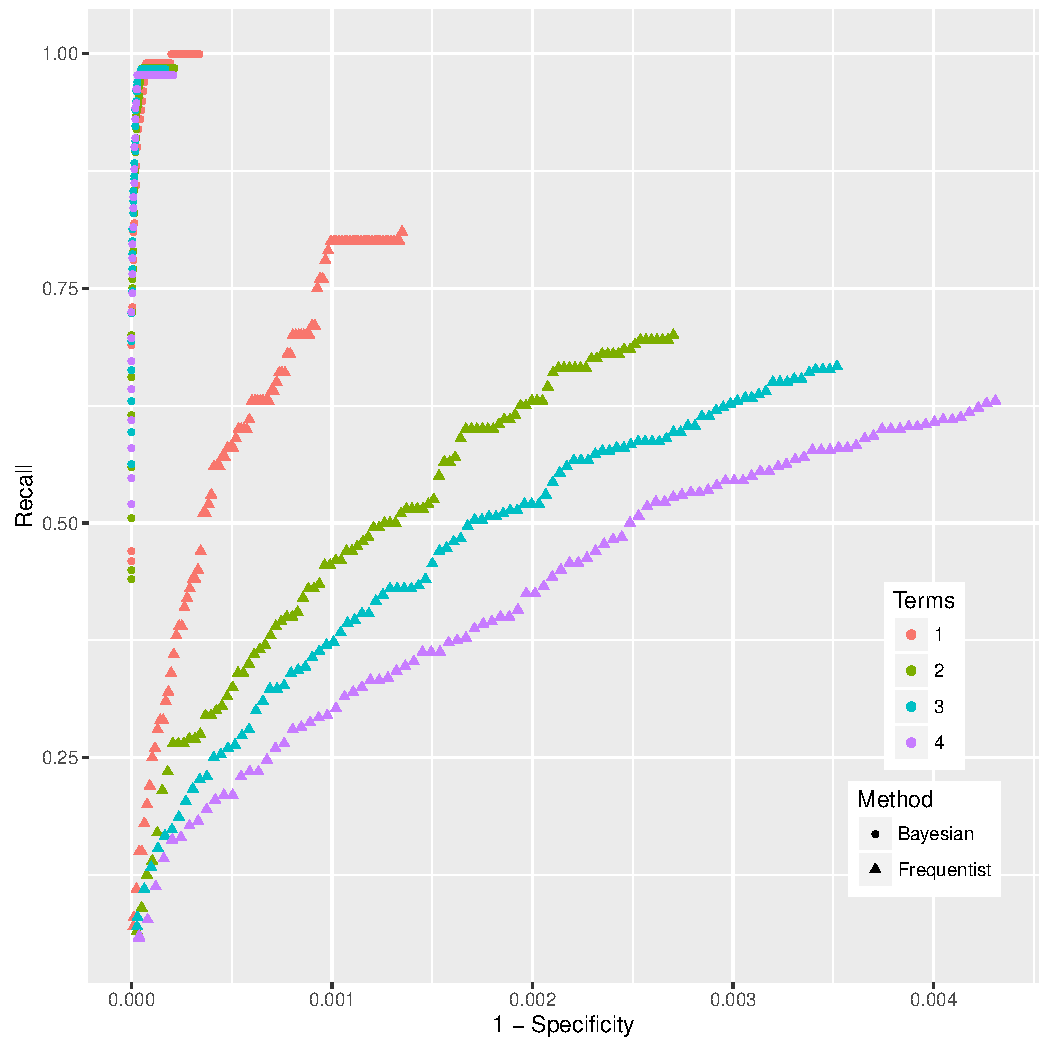
\includegraphics[width=\columnwidth]{allsim-color.pdf}
\caption{
  \label{fig:simresults}
  ROC curves for Frequentist and Bayesian TEA. The axes are scaled per term.
  There are 5,919 ontology terms annotated to {\em S.cerevisiae} genes, so (for example)
  a false discovery rate of 0.001 corresponds to about 6 falsely reported terms.
}
\end{figure}

We have implemented both Frequentist TEA (with Bonferroni correction) and Bayesian TEA (as described above), in both C++11 and JavaScript.
The JavaScript version can be run as a command-line tool using node, or via a web interface in a browser, and includes extensive unit tests.
The two implementations use the same random number generator and yield numerically identical results.
The C++ version is about twice as fast:
a benchmark of Bayesian TEA on a late-2014 iMac (4GHz Intel Core i7),
using the abovementioned 17 yeast mating genes and the relevant subset of 518 GO terms, run for 1,000 samples per term,
took 37.6 seconds of user time for the C++ implementation and 79.8 seconds in JavaScript.

By contrast, the Frequentist TEA approach is almost instant.
However, its weaker statistical power is apparent from Figure~\ref{fig:simresults},
which compares the recall {\em vs} specificity of Bayesian and Frequentist methods
on simulated datasets. For values of $N$ from 1 to 4, we sampled $N$ terms
from the {\em S.cerevisiae} subset of the Gene Ontology,
and generated a corresponding set of yeast genes with false positive rate 0.1\% and false negative rate 1\%.
The MCMC sampler was run for 100 iterations per term, and this experiment was repeated 100 times.
The model-based approach has vastly superior recall to the Fisher exact test, and the difference
grows with the number of terms.


\bibliographystyle{natbib}
\bibliography{references}

\end{document}
